\documentclass[10pt]{article}
\usepackage{icmlko}

\icmlmeta{IP 파운데이션 월드모델}{51}{주고 받은 것이 정확히 같았다}{축 하나를 켜자 대상 다섯 셀이 오른 만큼 출처 다섯 셀이 내렸다 --- 상충을 처음으로 셀 단위에서 본다}

\begin{document}

\twocolumn[
\icmlheader

\begin{abstract}
노트 50은 펀딩 창작자 이력이 라벨과 $-$0.011로 무효라고 하고 ``시장의 성질''로
읽었다 --- 크라우드펀딩은 신인과 베테랑이 구분되지 않는다고. 같은 노트에 반증
조건을 적었다: ``다른 방식으로 이력을 재 신호가 나오면 축을 잘못 잰 것이다.''
캐시된 목록 3,876쪽에 프로젝트별 모금액과 성공 여부가 이미 있어 재요청 없이
여덟 가지로 다시 쟀다. \textbf{반증됐다} --- 사전 건수는 $-$0.018인데 \textbf{앞선
프로젝트의 최대 후원자 수는 $+$0.180}이다. 그리고 금액이 아니라 사람 수다
(최대 모금액 $+$0.047 대 최대 후원자 $+$0.180). \textbf{이월되는 것은 자본이
아니라 팬이다.} 그런데 축으로 켜니 서른 셀 평균이 $+$0.3478에서 $+$0.3487로
꿈쩍하지 않는다. 셀을 나눠 보고 이유를 알았다. \textbf{펀딩이 대상인 다섯 셀이
$+$0.2141에서 $+$0.2623으로 오르고(+0.048), 출처인 다섯 셀이 $+$0.3851에서
$+$0.3423으로 내린다($-$0.043).} 노트 38·40의 상충 법칙이 축 하나를 켜는 것만으로
재현되고, 이번에는 \emph{정확히 상쇄}된다. 역할별로 나눠 주면 둘 다 얻을 수
있으므로 노트 39의 이중 배선을 다시 시험했다 --- 점추정은 세 방식 중 최고
($+$0.3559)인데 짝지은 구간이 {[}$-$0.013, $+$0.007{]}로 0을 포함한다(P$=$0.395).
\textbf{상충은 실재하고, 그것을 우회해서 얻는 몫은 현재 표본에서 잴 수 없는
크기다.}
\end{abstract}
]

\section{반증 조건이 발동했다}

노트 50은 펀딩 창작자 이력을 \emph{건수}로만 셌다. 캐시된 목록에 프로젝트마다
모금액·후원자 수·성공 여부가 들어 있으므로 재요청 없이 여덟 가지로 다시 쟀다.

\begin{figure}[t]
\centering
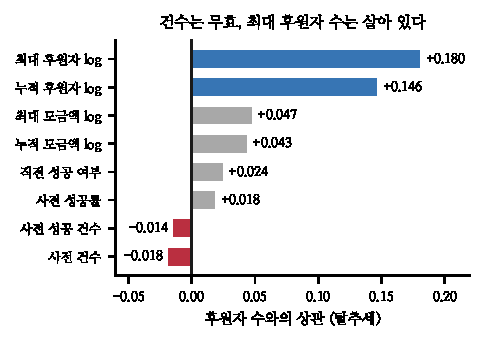
\includegraphics[width=\columnwidth]{figs/prior.pdf}
\caption{창작자 사전 이력을 재는 여덟 방식.}
\end{figure}

\begin{table}[t]
\centering\tsize
\caption{펀딩 사전 이력과 후원자 수의 상관(탈추세). 이력 있는 것 285/400건.}
\begin{tabular}{lr}
\toprule
방식 & r \\
\midrule
\textbf{최대 후원자 수 log} & \textbf{$+$0.180} \\
누적 후원자 수 log & $+$0.146 \\
최대 모금액 log & $+$0.047 \\
누적 모금액 log & $+$0.043 \\
직전 성공 여부 & $+$0.024 \\
사전 성공률 & $+$0.018 \\
사전 성공 건수 & $-$0.014 \\
사전 건수(노트 50) & $-$0.018 \\
\bottomrule
\end{tabular}
\end{table}

\claimx{크라우드펀딩에서 창작자 이력은 통한다. 다만 \emph{몇 번 했느냐}가 아니라
\emph{가장 크게 닿은 것이 얼마나 컸느냐}이고, 금액이 아니라 사람 수다. 이월되는
것은 자본이 아니라 팬이다.}{최대 후원자 수가 앞선 프로젝트의 규모가 아니라 그
창작자의 활동 기간을 대리하는 것일 수 있다. 기간을 통제하고도 남는지 보지 않았다.}

노트 50의 ``시장 성질'' 해석을 \textbf{부분 철회한다}. 이력이 안 통하는 시장이
아니라 이력을 잘못 재고 있었다. 다만 여섯 도메인 스펙트럼($+$0.322에서
$-$0.011까지)이 측정 방식 차이도 포함한다는 것이 여기서 드러났으므로, 그
비교 자체가 약해진다.

\paragraph{라벨을 사람 수로 고른 것이 값을 했다}
노트 40에서 펀딩 라벨을 모금액이 아니라 후원자 수로 정했다 --- 팝업 방문자와
같은 물리량이어야 한다는 이유였다. 이력에서도 사람 수가 금액을 네 배 앞선다.
같은 물리량으로 재는 것이 두 자리에서 이득이었다.

\section{그런데 축은 꿈쩍하지 않는다}

\begin{table}[t]
\centering\tsize
\caption{최대 후원자 수를 매장 노출도 축으로 켠 결과.}
\begin{tabular}{lr}
\toprule
설정 & 서른 셀 평균 $\rho$ \\
\midrule
끔(현행) & $+$0.3478 \\
켬 & $+$0.3487 \\
\bottomrule
\end{tabular}
\end{table}

단독 상관 $+$0.180인데 $\Delta+0.0009$다. 노트 37에서 게임 가격($+$0.351)을
켰다가 성적이 떨어진 것과 같은 종류이며, 여섯 도메인 · 순위 기준에서 세 번째
사례다.

\section{셀을 나누니 정확히 상쇄였다}

\begin{figure}[t]
\centering
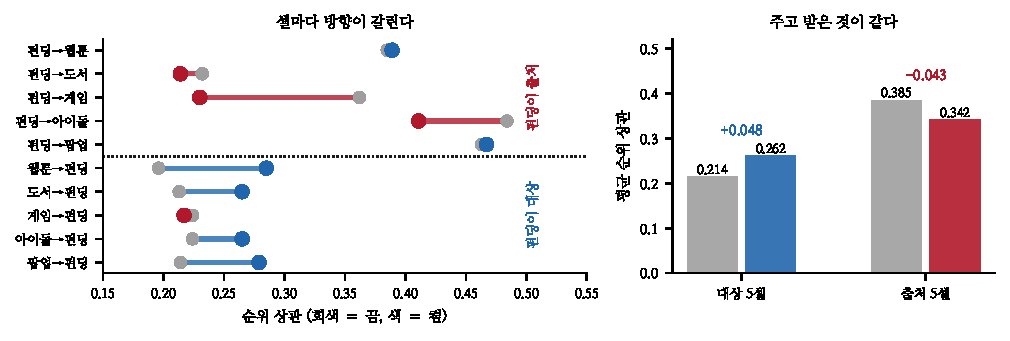
\includegraphics[width=\textwidth]{figs/exact.pdf}
\caption{왼쪽 --- 열 셀 각각. 오른쪽 --- 역할별 평균.}
\end{figure}

\begin{table}[t]
\centering\tsize
\caption{펀딩이 낀 열 셀.}
\begin{tabular}{lrrr}
\toprule
& 끔 & 켬 & $\Delta$ \\
\midrule
\textbf{펀딩이 대상} (5셀) & $+$0.2141 & $+$0.2623 & \textbf{$+$0.048} \\
\textbf{펀딩이 출처} (5셀) & $+$0.3851 & $+$0.3423 & \textbf{$-$0.043} \\
\midrule
열 셀 평균 & $+$0.2996 & $+$0.3023 & $+$0.003 \\
나머지 스무 셀 & $+$0.3720 & $+$0.3720 & 0.000 \\
\bottomrule
\end{tabular}
\end{table}

\claimx{축 하나를 켜는 것만으로 상충이 셀 단위에서 나타나고, 이번 경우 주고
받은 것이 정확히 같다($+$0.048 대 $-$0.043). 도메인에 정보를 더하면 그 도메인을
예측하기는 쉬워지고 그 도메인으로 가르치기는 어려워진다.}{다른 축에서도 상쇄가
이만큼 정확하면 우연이 아니다. 지금은 한 사례다.}

가장 큰 개별 변화가 펀딩$\to$게임의 $-$0.131이다. 그 셀은 정렬 축이 둘로
그대로인데(게임이 공통 축 둘만 관측한다) 펀딩 쪽 인자 공간이 바뀌어 계수가
어긋난다.

\section{나눠 주면 되지 않나}

역할에 따라 다른 배선을 쓰면 대상 쪽 이득만 취하고 출처 쪽 손해를 피할 수 있다.
노트 39가 만들었다가 노트 43에서 철회한 이중 배선이다. 여기서는 상충이 셀
단위로 문서화돼 있으니 다시 시험할 값이 있다.

\begin{table}[t]
\centering\tsize
\caption{펀딩 매장 노출도의 세 가지 운용.}
\begin{tabular}{lr}
\toprule
& 서른 셀 평균 $\rho$ \\
\midrule
끔 & $+$0.3478 \\
켬 & $+$0.3487 \\
\textbf{이중}(대상일 때만 켬) & \textbf{$+$0.3559} \\
\midrule
이중 $-$ 끔 & $+$0.0080 \\
짝지은 95\% 구간 & $[-0.013,\ +0.007]$ \\
P($>$0) & 0.395 \\
\bottomrule
\end{tabular}
\end{table}

점추정은 셋 중 최고인데 구간이 0을 포함하고 P가 0.395다. 구간 상한($+$0.007)이
점추정($+$0.008)보다 낮은 것도 붓스트랩이 한쪽으로 치우쳤다는 신호다.
\textbf{보류하고 노트 43의 철회를 유지한다.}

\begin{quote}\fontsize{9.5}{11.5}\selectfont
상충은 실재한다 --- 셀 단위로 $+$0.048 대 $-$0.043까지 봤다. 그런데 그것을
우회해서 얻는 몫은 서른 셀 평균으로 $+$0.008이고, 현재 구간 반폭이 0.056이다.
\textbf{실재하는 것과 측정할 수 있는 것이 다르다.}
\end{quote}

\section{한계}

\begin{itemize}[leftmargin=1.1em,itemsep=0.15em]
\item 최대 후원자 수가 창작자의 활동 기간을 대리할 수 있다. 기간을 통제하지
      않았다.
\item 상쇄가 정확한 것은 한 사례다. 다른 축에서 재현되는지 보지 않았다.
\item 이중 배선을 대상 쪽만 켜는 형태로 시험했다. 출처 쪽만 켜거나 둘 다 다른
      변수를 쓰는 조합은 안 봤다.
\item 펀딩$\to$게임 $-$0.131의 원인을 계수 어긋남으로 추측만 했다.
\item 노트 50의 여섯 도메인 스펙트럼이 측정 방식 차이를 포함한다는 것이
      드러났는데, 다른 다섯 도메인의 이력을 최대 후원자 수에 해당하는 방식으로
      다시 재지 않았다.
\end{itemize}

\section{다음}

\begin{enumerate}[leftmargin=1.3em,itemsep=0.15em]
\item 다른 다섯 도메인의 이력도 ``최대 규모''로 다시 잰다 --- 아이돌 소속사의
      최대 초동, 출판사의 최대 판매지수처럼. 노트 50의 스펙트럼을 공정하게
      다시 그린다.
\item 상쇄의 정확성을 다른 축에서 확인한다.
\item 최대 후원자 수에서 활동 기간을 통제한다.
\item 큰 도메인을 늘려 구간을 좁힌다 --- 이중 배선 같은 $+$0.008급 결정을
      판정하려면 반폭이 0.02 아래여야 한다.
\end{enumerate}

\vspace{0.6em}
\hrule height 0.3pt
\vspace{0.5em}
{\footnotesize
\textbf{참고문헌}\\[0.3em]
Merton, R. K. (1968). The Matthew effect in science. \emph{Science},
159(3810), 56--63.\\[0.15em]
Salganik, M. J., Dodds, P. S., Watts, D. J. (2006). Experimental study of
inequality and unpredictability in an artificial cultural market.
\emph{Science}, 311(5762), 854--856.\\[0.15em]
Standley, T. et al. (2020). Which tasks should be learned together in multi-task
learning? \emph{ICML}, 9120--9132.\\[0.15em]
Efron, B., Tibshirani, R. J. (1993). \emph{An Introduction to the Bootstrap}.
Chapman \& Hall.\\[0.15em]
Ben-David, S. et al. (2010). A theory of learning from different domains.
\emph{Machine Learning}, 79(1--2), 151--175.
}

\end{document}
